\documentclass{article}\usepackage[]{graphicx}\usepackage[]{color}
%% maxwidth is the original width if it is less than linewidth
%% otherwise use linewidth (to make sure the graphics do not exceed the margin)
\makeatletter
\def\maxwidth{ %
  \ifdim\Gin@nat@width>\linewidth
    \linewidth
  \else
    \Gin@nat@width
  \fi
}
\makeatother

\definecolor{fgcolor}{rgb}{0.345, 0.345, 0.345}
\newcommand{\hlnum}[1]{\textcolor[rgb]{0.686,0.059,0.569}{#1}}%
\newcommand{\hlstr}[1]{\textcolor[rgb]{0.192,0.494,0.8}{#1}}%
\newcommand{\hlcom}[1]{\textcolor[rgb]{0.678,0.584,0.686}{\textit{#1}}}%
\newcommand{\hlopt}[1]{\textcolor[rgb]{0,0,0}{#1}}%
\newcommand{\hlstd}[1]{\textcolor[rgb]{0.345,0.345,0.345}{#1}}%
\newcommand{\hlkwa}[1]{\textcolor[rgb]{0.161,0.373,0.58}{\textbf{#1}}}%
\newcommand{\hlkwb}[1]{\textcolor[rgb]{0.69,0.353,0.396}{#1}}%
\newcommand{\hlkwc}[1]{\textcolor[rgb]{0.333,0.667,0.333}{#1}}%
\newcommand{\hlkwd}[1]{\textcolor[rgb]{0.737,0.353,0.396}{\textbf{#1}}}%

\usepackage{framed}
\makeatletter
\newenvironment{kframe}{%
 \def\at@end@of@kframe{}%
 \ifinner\ifhmode%
  \def\at@end@of@kframe{\end{minipage}}%
  \begin{minipage}{\columnwidth}%
 \fi\fi%
 \def\FrameCommand##1{\hskip\@totalleftmargin \hskip-\fboxsep
 \colorbox{shadecolor}{##1}\hskip-\fboxsep
     % There is no \\@totalrightmargin, so:
     \hskip-\linewidth \hskip-\@totalleftmargin \hskip\columnwidth}%
 \MakeFramed {\advance\hsize-\width
   \@totalleftmargin\z@ \linewidth\hsize
   \@setminipage}}%
 {\par\unskip\endMakeFramed%
 \at@end@of@kframe}
\makeatother

\definecolor{shadecolor}{rgb}{.97, .97, .97}
\definecolor{messagecolor}{rgb}{0, 0, 0}
\definecolor{warningcolor}{rgb}{1, 0, 1}
\definecolor{errorcolor}{rgb}{1, 0, 0}
\newenvironment{knitrout}{}{} % an empty environment to be redefined in TeX

\usepackage{alltt}
\usepackage{natbib}
\usepackage{amsmath}
\usepackage{amssymb}
\usepackage{verbatim}
\usepackage{mathpazo}
\usepackage{setspace}
\usepackage[unicode=true]{hyperref}
\usepackage{geometry}
\geometry{tmargin=1in,bmargin=1in,lmargin=1in,rmargin=1in}

%% for inline R code: if the inline code is not correctly parsed, you will see a message
\newcommand{\rinline}[1]{SOMETHING WRONG WITH knitr}



\IfFileExists{upquote.sty}{\usepackage{upquote}}{}
\begin{document}
\title{Adaptive rejection sampling algorithm project}
\author{Lauren Ponisio, Katherine Ullman, Xinyue Zhou and Cenzhuo Yao}

\maketitle

Github repository for the final project is under username z35712526

\section{Approach}

We have two main objects that we create and update in our
function. The first is the $info$ matrix which stores the proposed
sample ($x$), the function evaluated at x, and the derivative of the
function evaluated at x. The second is $ret$ which stores accepted
samples values and is returned. 

We begin by creating our empty $info$ matrix using the approximation
for the number of iterations from Gilks et al.~1992. We then fill it
with initial values supplied by the user or by values or the defaults
of -inf to inf.

\begin{knitrout}
\definecolor{shadecolor}{rgb}{0.969, 0.969, 0.969}\color{fgcolor}\begin{kframe}
\begin{alltt}
\hlcom{## function for initialize the info matrix in unbounded cases}
\hlcom{## aa and bb are the bounds, info is the info matrix with x, fx, and}
\hlcom{## f'x, FUN is the function of interest and DD is the derivative}
\hlcom{## function}
\hlcom{## the function returns the updated info matrix}
\hlstd{help_init_info} \hlkwb{<-} \hlkwa{function} \hlstd{(}\hlkwc{aa}\hlstd{,} \hlkwc{bb}\hlstd{,} \hlkwc{info}\hlstd{,} \hlkwc{FUN}\hlstd{,} \hlkwc{DD}\hlstd{)\{}
  \hlstd{info[}\hlnum{1}\hlstd{,} \hlnum{1}\hlstd{]} \hlkwb{<-} \hlstd{aa}
  \hlstd{info[}\hlnum{1}\hlstd{,} \hlnum{2}\hlstd{]} \hlkwb{<-} \hlkwd{FUN}\hlstd{(info[}\hlnum{1}\hlstd{,} \hlnum{1}\hlstd{])}
  \hlkwa{if}\hlstd{(}\hlopt{!}\hlkwd{is.finite}\hlstd{(info[}\hlnum{1}\hlstd{,} \hlnum{2}\hlstd{])) \{}
    \hlkwd{stop}\hlstd{(}\hlstr{'aa is not defined on f'}\hlstd{,} \hlkwc{call.} \hlstd{=} \hlnum{FALSE}\hlstd{)}
  \hlstd{\}}
  \hlstd{info[}\hlnum{1}\hlstd{,} \hlnum{3}\hlstd{]} \hlkwb{<-} \hlkwd{DD}\hlstd{(info[}\hlnum{1}\hlstd{,} \hlnum{1}\hlstd{])}
  \hlstd{info[}\hlnum{2}\hlstd{,} \hlnum{1}\hlstd{]} \hlkwb{<-} \hlstd{bb}
  \hlstd{info[}\hlnum{2}\hlstd{,} \hlnum{2}\hlstd{]} \hlkwb{<-} \hlkwd{FUN}\hlstd{(info[}\hlnum{2}\hlstd{,} \hlnum{1}\hlstd{])}
  \hlkwa{if}\hlstd{(}\hlopt{!}\hlkwd{is.finite}\hlstd{(info[}\hlnum{1}\hlstd{,} \hlnum{2}\hlstd{])) \{}
    \hlkwd{stop}\hlstd{(}\hlstr{'bb is not defined on f'}\hlstd{,} \hlkwc{call.} \hlstd{=} \hlnum{FALSE}\hlstd{)}
  \hlstd{\}}
  \hlstd{info [}\hlnum{2}\hlstd{,} \hlnum{3}\hlstd{]} \hlkwb{<-} \hlkwd{DD}\hlstd{(bb)}
  \hlkwd{return}\hlstd{(info)}
\hlstd{\}}
\end{alltt}
\end{kframe}
\end{knitrout}

We then set our counters and enter a while loop.


Within the while loop we first check to see if the function is
log-concave using the $check\_concave$ function. That function checks
if the derivative of the function of interest evaluated at the
proposed samples is always decreasing. 

\begin{knitrout}
\definecolor{shadecolor}{rgb}{0.969, 0.969, 0.969}\color{fgcolor}\begin{kframe}
\begin{alltt}
\hlcom{## checks log-convexity}
\hlcom{## clean_info is the ordered info matrix}
\hlstd{check_concave} \hlkwb{<-} \hlkwa{function}\hlstd{(}\hlkwc{clean_info}\hlstd{)\{}
  \hlkwa{if}\hlstd{(}\hlkwd{is.null}\hlstd{(clean_info[,}\hlnum{3}\hlstd{])) \{}\hlkwd{return}\hlstd{(}\hlnum{TRUE}\hlstd{)\}}
  \hlkwd{return}\hlstd{(}\hlkwd{prod}\hlstd{(}\hlkwd{round}\hlstd{(clean_info[,}\hlnum{3}\hlstd{][}\hlopt{-}\hlnum{1}\hlstd{],}\hlnum{5}\hlstd{)} \hlopt{<=}
              \hlkwd{round}\hlstd{(clean_info[,}\hlnum{3}\hlstd{][}\hlopt{-}\hlkwd{nrow}\hlstd{(clean_info)],} \hlnum{5}\hlstd{)))}
\hlstd{\}}
\end{alltt}
\end{kframe}
\end{knitrout}

Next, a new proposed sample is taken ($x$) using
$sample\_envelope$. The function draws two random uniform numbers. The
first draw is to determine which piece of the upper bound to sample
from. The second draw is to calculate the sample $x$ by evaluating
the inverse cdf at the value of the random draw. The function returns
the proposed sample.


\begin{knitrout}
\definecolor{shadecolor}{rgb}{0.969, 0.969, 0.969}\color{fgcolor}\begin{kframe}
\begin{alltt}
\hlcom{## returns a new sample given the info matrix and z}
\hlcom{## input is clean info matrix and clean z}
\hlstd{sample_envelope} \hlkwb{<-} \hlkwa{function}\hlstd{(}\hlkwc{samp_info}\hlstd{,} \hlkwc{samp_z}\hlstd{,} \hlkwc{num_sample}\hlstd{)\{}
  \hlcom{## segments of bounds}
  \hlstd{p} \hlkwb{<-} \hlkwd{rep}\hlstd{(}\hlnum{NA}\hlstd{,} \hlkwd{nrow}\hlstd{(samp_info))}
  \hlstd{p} \hlkwb{<-} \hlkwd{exp}\hlstd{(samp_info[,}\hlnum{2}\hlstd{])}\hlopt{*}\hlstd{(}\hlkwd{exp}\hlstd{((samp_z[}\hlopt{-}\hlnum{1}\hlstd{]} \hlopt{-} \hlstd{samp_info[,}\hlnum{1}\hlstd{])}\hlopt{*}
                               \hlstd{samp_info[,}\hlnum{3}\hlstd{])} \hlopt{-}
                           \hlkwd{exp}\hlstd{((samp_z[}\hlopt{-}\hlkwd{nrow}\hlstd{(samp_info)} \hlopt{-} \hlnum{1}\hlstd{]} \hlopt{-}
                                \hlstd{samp_info[,}\hlnum{1}\hlstd{])}\hlopt{*}
                               \hlstd{samp_info[,}\hlnum{3}\hlstd{]))}\hlopt{/}\hlstd{samp_info[,}\hlnum{3}\hlstd{]}
  \hlcom{## q for normalizing p}
  \hlstd{q} \hlkwb{<-} \hlstd{p}\hlopt{/}\hlkwd{sum}\hlstd{(p)}
  \hlcom{## which region we sample from}
  \hlstd{w} \hlkwb{<-} \hlkwd{runif}\hlstd{(num_sample)}
  \hlstd{i} \hlkwb{<-} \hlkwd{vector}\hlstd{(}\hlkwc{mode} \hlstd{=} \hlstr{'numeric'}\hlstd{,} \hlkwc{length} \hlstd{= num_sample)}
  \hlkwa{for} \hlstd{(j} \hlkwa{in} \hlnum{1}\hlopt{:}\hlstd{num_sample)\{}
    \hlstd{i[j]} \hlkwb{<-} \hlkwd{sum}\hlstd{(}\hlkwd{cumsum}\hlstd{(q)} \hlopt{<} \hlstd{w[j])} \hlopt{+} \hlnum{1}
  \hlstd{\}}
  \hlcom{## sample pi using inv cdf}
  \hlstd{samp_x} \hlkwb{<-} \hlstd{(}\hlkwd{log}\hlstd{(p[i]}\hlopt{*}\hlkwd{runif}\hlstd{(num_sample)}\hlopt{*}\hlstd{samp_info[i,} \hlnum{3}\hlstd{]} \hlopt{+}
                   \hlkwd{exp}\hlstd{(samp_info[i,}\hlnum{2}\hlstd{]} \hlopt{+}
                         \hlstd{(samp_z[i]} \hlopt{-} \hlstd{samp_info[i,}\hlnum{1}\hlstd{])}\hlopt{*}\hlstd{samp_info[i,}\hlnum{3}\hlstd{]))} \hlopt{-}
               \hlstd{samp_info[i,}\hlnum{2}\hlstd{])}\hlopt{/}\hlstd{samp_info[i,}\hlnum{3}\hlstd{]} \hlopt{+} \hlstd{samp_info[i,}\hlnum{1}\hlstd{]}
  \hlkwd{return}\hlstd{(samp_x)}
\hlstd{\}}
\end{alltt}
\end{kframe}
\end{knitrout}

We then check if it is defined on the function of interest and draw a
new x if it is not. We also check whether $x$ has already been drawn
and save it in the output if it has been.

We then draw a $w$ from the uniform(0,1) that will be used to identify
whether the sample is accepted or rejected.

We next calculate the lower bound using the function $line\_fun$ which
takes two points and calculates the slope between those points, and
evaluations that line function to return the y value.

\begin{knitrout}
\definecolor{shadecolor}{rgb}{0.969, 0.969, 0.969}\color{fgcolor}\begin{kframe}
\begin{alltt}
\hlcom{## takes two points and returns the function of that line}
\hlstd{line_fun} \hlkwb{<-} \hlkwa{function}\hlstd{(}\hlkwc{x1}\hlstd{,} \hlkwc{y1}\hlstd{,} \hlkwc{x2}\hlstd{,} \hlkwc{y2}\hlstd{,} \hlkwc{x_star}\hlstd{)\{}
  \hlkwa{if}\hlstd{(x1} \hlopt{==} \hlstd{x2) \{}\hlkwd{stop}\hlstd{(}\hlstr{'Two points in a vertical line'}\hlstd{)\}}
  \hlstd{y_star} \hlkwb{<-} \hlstd{(y2} \hlopt{-} \hlstd{y1)}\hlopt{/}\hlstd{(x2} \hlopt{-} \hlstd{x1)}\hlopt{*}\hlstd{(x_star} \hlopt{-} \hlstd{x1)} \hlopt{+} \hlstd{y1}
  \hlkwd{return}\hlstd{(y_star)}
\hlstd{\}}
\end{alltt}
\end{kframe}
\end{knitrout}

For the upper bound, we only have one point and the derivative,
so we used the function $line\_fun\_p$ to evaluate the line at that
point.

We then determine whether our sample:
\begin{enumerate}
\item falls within the lower bound. If it does, we accept it and store
it in $ret$
\item falls between the lower bound and the function of interest.  If
it does, we accept it and store it in $ret$. We also evaluate the
function and its derivative at the sample and update the $info$ matrix
using $update\_info$ function.
\item falls between the function and the upper bound. If it does, we
reject the sample. We also again update the $info$ matrix.
\end{enumerate}

We continue in the while loop until the desired number of accepted
samples is reached. 

\subsection{Special cases}

For the uniform distribution, the derivative is always zero. If for the
bounded uniform, the derivative at both of the provided initial
condition is zero, it must be the uniform so we just draw using $runif$.

\subsection{Numerical differentiation}

We created a function for numerical differentiation. 

We choose $\epsilon$ to be $1^{-8}$ and then evaluated:
\begin{equation}
\label{eq:deriv}
f' \propto (f(x+\epsilon) + f(x-\epsilon))/2\epsilon  \\
\end{equation}

Or at the boundaries:
\begin{equation}
\label{eq:deriv}
f' \propto (f(x) + f(x-\epsilon))/\epsilon  \\ 
\end{equation}

\begin{equation}
\label{eq:deriv}
f' \propto (f(x+\epsilon) + f(x))/\epsilon  \\ 
\end{equation}

\begin{knitrout}
\definecolor{shadecolor}{rgb}{0.969, 0.969, 0.969}\color{fgcolor}\begin{kframe}
\begin{alltt}
\hlcom{## function for numerically approximating the derivative}
\hlcom{## x is the point to evaluate the derivate at, FUN is the function,}
\hlcom{## a and b are the bounds}
\hlcom{## the function returns the approximation to the derivative at the point of}
\hlcom{## evaluation}
\hlstd{Derv} \hlkwb{<-} \hlkwa{function}\hlstd{(}\hlkwc{x}\hlstd{,} \hlkwc{FUN}\hlstd{,} \hlkwc{a}\hlstd{,} \hlkwc{b}\hlstd{)\{}
  \hlkwa{if} \hlstd{(x} \hlopt{==} \hlstd{a) \{}\hlkwd{return} \hlstd{((}\hlkwd{FUN}\hlstd{(x} \hlopt{+} \hlnum{1e-8}\hlstd{)}\hlopt{-}\hlkwd{FUN}\hlstd{(x))}\hlopt{/}\hlnum{1e-8}\hlstd{)\}}
  \hlkwa{if} \hlstd{(x} \hlopt{==} \hlstd{b) \{}\hlkwd{return} \hlstd{((}\hlkwd{FUN}\hlstd{(x)} \hlopt{-} \hlkwd{FUN}\hlstd{(x} \hlopt{-} \hlnum{1e-8}\hlstd{))}\hlopt{/}\hlnum{1e-8}\hlstd{)\}}
  \hlkwa{if} \hlstd{(a} \hlopt{<=} \hlstd{x} \hlopt{&&} \hlstd{x} \hlopt{<=} \hlstd{b) \{}\hlkwd{return}\hlstd{((}\hlkwd{FUN}\hlstd{(x} \hlopt{+} \hlnum{1e-8}\hlstd{)}\hlopt{-}\hlkwd{FUN}\hlstd{(x} \hlopt{-} \hlnum{1e-8}\hlstd{))}\hlopt{/}\hlnum{2e-8}\hlstd{)\}}
\hlstd{\}}
\end{alltt}
\end{kframe}
\end{knitrout}

\subsection{Efficiency}

\subsubsection{Vectorization}
All of the algorithm is vectorized. 

\subsubsection{Sorting}
After each update, we needed to re-sort the $info$ matrix and $z$
vector. Instead of using the build-in $sort()$ function, we just found
the index where the new value needed to be added.

\subsubsection{Sampling in batches}
After originally sampling, one value at a time, we extended the
function to sample batches of proposed samples at a time.

We had to decide when it was most efficient to take one sample at a
time and update the bounds, or draw multiple samples. We decided to
first look at the $hit\_rate$, which is the number of accepted samples
out of the number of total draws. When $hit\_rate=1$, this means that
we have not updated our bounds. This is because we are early in our
iterations and do not have a good approximation of our function. So,
if $hit\_rate=1$, we draw one sample at a time. If the $hit\_rate$ is
close to 1, it means that most of the samples we draw will go to
sample and thus our approximation of the function with the upper bound
and lower bound is good. If $hit\_rate < 1$, we draw $1/(1 - hit\_rate)$
sample at a time.

\section{Testing}

\subsection{Final tests} To test our algorithm we compared our samples
to known distributions using Kolmogorov-Smirnov test. We tested our
function against known log-concave distributions including the normal,
gamma, Laplace, logistic, beta and uniform (Fig.~\ref{fig:dists}).

Our algorithm consistently passes for all of the functions. Sometimes
the samples did fail however, likely because the numerical
differentiation does not preform well.

\subsection{Defensive programming}

We created to checks to determine whether the inputs arguments were in
the expected format. We also checked if the derivative function provide
by the user was the correct derivative function. 

We also created a function that checks whether the input function is
log-concave by checking whether the derivative is always
decreasing. We added checks for when the function was not defined
on the sample.

\subsection{Unit tests}

We used Browser() to do informal testing of each module. Because our
modules were all uncomplicated (most sort objects and do basic
arithmetic), we could not think of sensible formal tests to
perform for most of the modules. We performed a unit test for the most
complex function, $sample\_envelope$ using the exponential.

Because the exponential distribution is fairly simple, we could create
an $info$ matrix and $z$ vector that encompassed the entire
distribution. Therefore we could compare the samples from
$sample\_envelope$ to the theoretical exponential using a
Kolmogorov-Smirnov test. 

\begin{knitrout}
\definecolor{shadecolor}{rgb}{0.969, 0.969, 0.969}\color{fgcolor}\begin{kframe}
\begin{alltt}
\hlstd{sample_envelope} \hlkwb{<-} \hlkwa{function}\hlstd{(}\hlkwc{samp_info}\hlstd{,} \hlkwc{samp_z}\hlstd{,} \hlkwc{num_sample}\hlstd{)\{}
  \hlcom{## segments of bounds}
  \hlstd{p} \hlkwb{<-} \hlkwd{rep}\hlstd{(}\hlnum{NA}\hlstd{,} \hlkwd{nrow}\hlstd{(samp_info))}
  \hlstd{p} \hlkwb{<-} \hlkwd{exp}\hlstd{(samp_info[,}\hlnum{2}\hlstd{])}\hlopt{*}\hlstd{(}\hlkwd{exp}\hlstd{((samp_z[}\hlopt{-}\hlnum{1}\hlstd{]} \hlopt{-} \hlstd{samp_info[,}\hlnum{1}\hlstd{])}\hlopt{*}
                               \hlstd{samp_info[,}\hlnum{3}\hlstd{])} \hlopt{-}
                           \hlkwd{exp}\hlstd{((samp_z[}\hlopt{-}\hlkwd{nrow}\hlstd{(samp_info)} \hlopt{-} \hlnum{1}\hlstd{]} \hlopt{-}
                                \hlstd{samp_info[,}\hlnum{1}\hlstd{])}\hlopt{*}
                               \hlstd{samp_info[,}\hlnum{3}\hlstd{]))}\hlopt{/}\hlstd{samp_info[,}\hlnum{3}\hlstd{]}
  \hlcom{## q for normalizing p}
  \hlstd{q} \hlkwb{<-} \hlstd{p}\hlopt{/}\hlkwd{sum}\hlstd{(p)}
  \hlcom{## which region we sample from}
  \hlstd{w} \hlkwb{<-} \hlkwd{runif}\hlstd{(num_sample)}
  \hlstd{i} \hlkwb{<-} \hlkwd{vector}\hlstd{(}\hlkwc{mode} \hlstd{=} \hlstr{'numeric'}\hlstd{,} \hlkwc{length} \hlstd{= num_sample)}
  \hlkwa{for} \hlstd{(j} \hlkwa{in} \hlnum{1}\hlopt{:}\hlstd{num_sample)\{}
    \hlstd{i[j]} \hlkwb{<-} \hlkwd{sum}\hlstd{(}\hlkwd{cumsum}\hlstd{(q)} \hlopt{<} \hlstd{w[j])} \hlopt{+} \hlnum{1}
  \hlstd{\}}
  \hlcom{## sample pi using inv cdf}
  \hlstd{samp_x} \hlkwb{<-} \hlstd{(}\hlkwd{log}\hlstd{(p[i]}\hlopt{*}\hlkwd{runif}\hlstd{(num_sample)}\hlopt{*}\hlstd{samp_info[i,} \hlnum{3}\hlstd{]} \hlopt{+}
                   \hlkwd{exp}\hlstd{(samp_info[i,}\hlnum{2}\hlstd{]} \hlopt{+}
                         \hlstd{(samp_z[i]} \hlopt{-} \hlstd{samp_info[i,}\hlnum{1}\hlstd{])}\hlopt{*}\hlstd{samp_info[i,}\hlnum{3}\hlstd{]))} \hlopt{-}
               \hlstd{samp_info[i,}\hlnum{2}\hlstd{])}\hlopt{/}\hlstd{samp_info[i,}\hlnum{3}\hlstd{]} \hlopt{+} \hlstd{samp_info[i,}\hlnum{1}\hlstd{]}
  \hlkwd{return}\hlstd{(samp_x)}
\hlstd{\}}


\hlcom{## test using the exponential}
\hlkwd{set.seed}\hlstd{(}\hlnum{4}\hlstd{)}
\hlstd{a} \hlkwb{<-} \hlnum{0}
\hlstd{b} \hlkwb{<-} \hlnum{1}
\hlstd{lambda} \hlkwb{<-} \hlnum{1}

\hlstd{samp_info} \hlkwb{<-} \hlkwd{matrix}\hlstd{(}\hlkwd{c}\hlstd{(a, b,}
                      \hlkwd{log}\hlstd{(}\hlkwd{dexp}\hlstd{(a,} \hlkwc{rate}\hlstd{=lambda)),}
                      \hlkwd{log}\hlstd{(}\hlkwd{dexp}\hlstd{(b,} \hlkwc{rate}\hlstd{= lambda)),}
                      \hlopt{-}\hlstd{lambda,}
                      \hlopt{-}\hlstd{lambda),} \hlkwc{nrow}\hlstd{=}\hlnum{2}\hlstd{)}
\hlstd{samp_z} \hlkwb{<-} \hlkwd{c}\hlstd{(}\hlnum{0}\hlstd{,} \hlnum{0.5}\hlstd{,} \hlnum{Inf}\hlstd{)}

\hlstd{test.out} \hlkwb{<-} \hlkwd{sample_envelope}\hlstd{(samp_info, samp_z,} \hlnum{10000}\hlstd{)}

\hlstd{out.test} \hlkwb{<-} \hlkwd{ks.test}\hlstd{(test.out, pexp)}

\hlkwa{if}\hlstd{(out.test}\hlopt{$}\hlstd{p.value} \hlopt{>} \hlnum{0.05}\hlstd{)\{}
  \hlkwd{print}\hlstd{(}\hlstr{"sample matches exponential, sample_envelope unit test passed"}\hlstd{)}
\hlstd{\}}\hlkwa{else}\hlstd{\{}
  \hlkwd{print}\hlstd{(}\hlstr{"sample does not match exponential, sample_envelope unit test failed"}\hlstd{)}
\hlstd{\}}
\end{alltt}
\begin{verbatim}
## [1] "sample matches exponential, sample_envelope unit test passed"
\end{verbatim}
\end{kframe}
\end{knitrout}

The real test is whether our overall function was able to
reproduce samples from known distribution, which was the case.

\section{Contributions} Zhou and Yao wrote the skeleton of the
algorithm, and all members contributed to de-bugging, improving
efficiency, and improving style. Zhou and Yao finalized the
functions. Lauren and Katherine wrote the testing functions, and wrote
the first draft of the write up. All members contributed to
revisions. Katherine wrote the help documentation. We worked together
to package the code into a package.

\clearpage

\begin{figure}
\centering
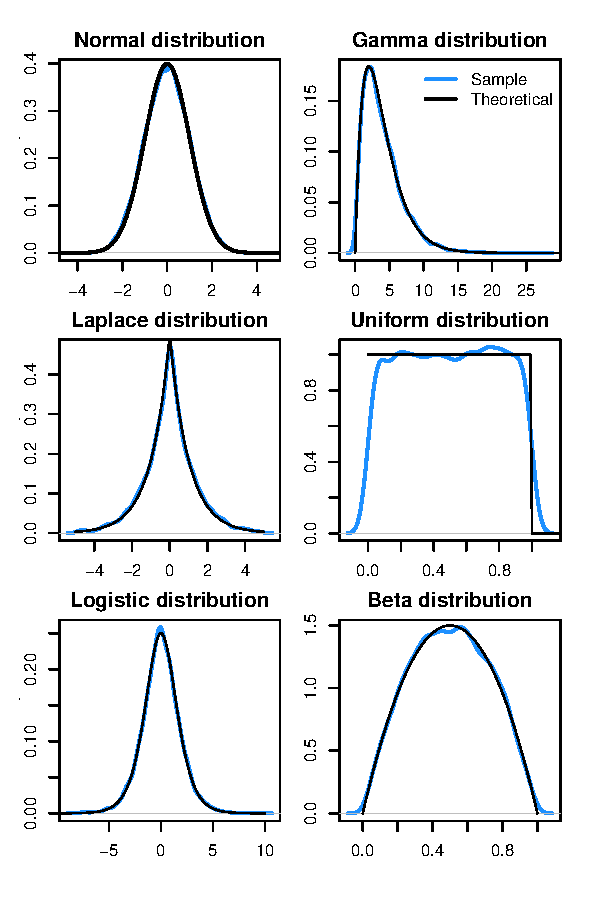
\includegraphics[width=0.8\textwidth]{figures/densities.pdf}
\caption{A comparison of the sample and theoretical pdfs for
different log-concave distributions.}
\label{fig:dists}
\end{figure}

\clearpage
\end{document}
